
\subsection{Jogosultságok}

\begin{itemize}
\item minden állománynak van tulajdonosa és csoportja 
\item mindezekhez tartozik 
	\begin{description}
	\item[r] olvasási jog

\begin{quotation}
\small		
	Ha a tulajdonosnak az olvasási jogát jelző kapcsoló be van kapcsolva, akkor az adott állományban található adatokat a tulajdonos megnézheti, olvashatja, kinyomtathatja, lemásolhatja, egy szóval az adatokhoz hozzáférhet. Ha e kapcsoló ki van kapcsolva, akkor az állomány nevét látja ugyan a tulajdonos, de a tartalmához nem férhet hozzá.


A \textit{könyvtáron értelmezett olvasási jog} a benne található állományok nevének kilistázását jelenti. Ha ezzel a joggal rendelkezik valaki akkor listázhatja az állományokat az adott könyvtárban, ha nem, akkor ezt nem teheti meg. Ötletes módon, az állományokat esetleg létrehozhatja, és akár módosíthatja is, attól függetlenül, hogy róluk listát nem kaphat.
\end{quotation}

	\item[w] írási jog

\begin{quotation}
\small	
	A tulajdonos írási jog kapcsolója megmutatja, hogy a számára engedélyezett-e az adatok írása, vagyis módosítása. Ha ez be van kapcsolva, akkor a tulajdonos módosíthatja, bővítheti és törölheti az adott állományban található adatokat, sőt törölheti akár az egész állományt. Ha e kapcsoló ki van kapcsolva, akkor a tulajdonos nem módosíthatja az adatokat, még az állomány végére sem fűzhet újabb információkat.
	
A \textit{könyvtáron értelmezett írási jog} újabb fájlok létrehozására és törlésére ad lehetőséget. Ha írási joggal nem rendelkezik valaki az adott könyvtárban, esetleg még írhat a benne levő állományokba vagy azokból adatokat törölhet. Egész állományokat nem hozhat létre és egész állományokat viszont nem törölhet. Amennyiben a könyvtárból az ott található állományokat nem tudja a felhasználó kitörölni, a könyvtárat magát sem tudja törölni, hiszen csak üres könyvtárakat lehet kitörölni. Ha a könyvtár már üres, a felhasználónak nincs szüksége írási jogra a könyvtárra nézve ahhoz, hogy azt kitörölhesse.
\end{quotation}


	\item[x] futtatási jog
	
\begin{quotation}
\small	
	A tulajdonos futtatási jogát jelzőkapcsoló azt mutatja meg, hogy a tulajdonos elindíthatja-e az adott állományt. Ennek a lehetőségnek csak programok esetében van értelme. %, adatokat tartalmazó állomány esetében e kapcsoló ki van kapcsolva.
	
A \textit{könyvtáron értelmezett futtatási jog} a könyvtár megnyitását jelenti, vagyis azt a képességet, hogy a könyvtárba belépjünk.


\end{quotation}
	\end{description}

\item fájl(ok) futtatásához és mappa megnyitáshoz is \texttt{rx} (olvasási és futtatási) jog szükséges
\end{itemize}
\bigskip

\noindent{\large\Ovalbox{\verb.chmod. - fájlok elérési jogainak megváltoztatása }
	\hfill \texttt{chmod +|-<mód> <fájlnév>}}
	\medskip
	
Egy fájl tulajdonosi (hozzáférési) jogait csak a fájl tulajdonosa, vagy a rendszergazda tudja megváltoztatni. A továbbiakban tegyük fel, hogy a \texttt{pelda.txt} file tulajdonosa  mi vagyunk.
\begin{description}
\item[+/-:] ezzel jelezzük, hogy adunk vagy elveszünk jogot.
\item[mód]: két dolgot kell ezesetben meghatároznunk\medskip

	\textit{kinek adunk}
	\begin{description}
	\item[u] pl. \texttt{chmod u+w pelda.txt} - saját magunknak írási jog
	\item[g] pl. \texttt{chmod g+r pelda.txt} - csoportnak olvasási jog
	\item[o] pl. \texttt{chmod o+x pelda.txt} - másoknak futtatási jog
	\item[a] (all -- mindenki)  \texttt{chmod a+rwx pelda.txt} - mindenkinek megadjuk az olvasási, írási és futtatási jogot
	\end{description}
	
	\textit{\dots és milyen jogot}
	\begin{description}
	\item[r,w,x] (lásd feljebb)
	\end{description}
	
	Lehet kombinálni is a fentieket, pl. \texttt{\$chmod ug+w pelda.txt}
\bigskip
	
Ha a csoportot -- akire az adott jog vonatkozik -- nem adjuk meg, akkor az mindhárom csoportra vonatkozik:
\begin{lstlisting}
joe@localhost:~$ ls -l fajl.txt 
-rw-r--r-- 1 joe joe 178 2011-02-11 18:45 fajl.txt
joe@localhost:~$ chmod +x fajl.txt
joe@localhost:~$ ls -l fajl.txt 
-rwxr-xr-x 1 joe joe 178 2011-02-11 18:45 fajl.txt	
\end{lstlisting}


Ha nem a \verb.+. vagy \verb.-. jeleket használjuk, hanem az \verb.=. jelet, akkor azok a jogok kapcsolódnak be, amelyeket felsorolunk, a többi pedig visszavonásra kerül:

\begin{lstlisting}
joe@localhost:~$ ls -l fajl.txt 
-rwxr--r-- 1 joe joe 178 2011-02-11 18:45 fajl.txt
joe@localhost:~$ chmod u=rw fajl.txt 
joe@localhost:~$ ls -l fajl.txt 
-rw-r--r-- 1 joe joe 178 2011-02-11 18:45 fajl.txt
\end{lstlisting}



\end{description}

A jogosultságok  megváltoztatásakor nem csak a fenti mód használható, hanem számszerű formátumban  is megadhatjuk a jogokat. 

A jobb oldalon látható táblázat adja meg melyik joghoz milyen szám tartozik. Ha több jogot szeretnénk alkalmazni, akkor össze kell adnunk az értékeket, például az 5 az olvasási és futtatási jogot jelenti, a 6 az olvasásit és írásit. 
\begin{center}
\small
\begin{tabular}{lccc}
\toprule
	Jogok 	&\bf u 		&\bf g 		&\bf o\\
	 	&tulajdonos 	&csoport	&mindenki más\\
\midrule
\bf Olvasás 	&r 		&r		&r\\
\bf Írás	&w 		&w 		&w\\
\bf Futtatás 	&x 		&x 		&x\\
\bottomrule

\end{tabular}
\hfill
\begin{tabular}{lccc}
\toprule
	Jogok 	&\bf u 		&\bf g 		&\bf o\\
	 	&tulajdonos 	&csoport	&mindenki más\\
\midrule
\bf Olvasás 	&4 		&4 		&4\\
\bf Írás	&2 		&2 		&2\\
\bf Futtatás 	&1 		&1 		&1\\
\bottomrule
\end{tabular}
\end{center}

\bigskip

\textit{Példák}
Az alábbi táblázatban az egymás mellett levő parancsok ekvivalensek.
\begin{center}
\begin{tabular}{l|l}
\toprule
chmod u=rw,g=r,o=r fajl.txt	& chmod 644 fajl.txt\\
chmod ugo=rw fajl.txt		& chmod 666 fajl.txt\\
chmod a=rwx fajl.txt		& chmod 777 fajl.txt\\
chmod ugo-rwx fajl.txt	 	& chmod 000 fajl.txt\\
\bottomrule
\end{tabular}
\end{center}
\bigskip

{
\noindent\Ovalbox{\large\verb.chown. - fájlok felhasználói és csoport tulajdonosának megváltoztatása}
\medskip

       \hfill \texttt{chown [ kapcsolók ] [ tulajdonos ][:[ csoport ]] file(ok)}
       }\bigskip
       
       
A \verb.chown. (change owner, tulajdonosváltás) parancs segítségével megváltoztathatjuk az állomány tulajdonosát és csoporttulajdonosát. Alapesetben -- ha csak a tulajdonost változtatjuk -- a parancsnak a tulajdonos nevét és az állománynevet kell megadnunk:

\begin{lstlisting}
joe@localhost:~$ ls -l fajl.txt 
-rw-r--r-- 1 joe    joe 178 2011-02-11 18:45 fajl.txt
joe@localhost:~$ chown andrea fajl.txt 
joe@localhost:~$ ls -l fajl.txt 
-rw-r--r-- 1 andrea joe 178 2011-02-11 18:45 fajl.txt
\end{lstlisting}

Ha a csoporttulajdonost is meg akarjuk változtatni, akkor a tulajdonos neve után kettősponttal elválasztva kell az új csoportot megadnunk:

\begin{lstlisting}
joe@localhost:~$ chown joe:csoportnev fajl.txt
joe@localhost:~$ ls -l fajl.txt 
-rw-r--r-- 1 joe csoportnev 178 2011-02-11 18:45 fajl.txt
\end{lstlisting}

\medskip
\textit{Kapcsolók}
\begin{description}
\item[-R] rekurzívan változtatja meg a (paraméterként megadott) könyvtár és annak tartalmának tulajdonosát
\end{description}
\bigskip

\noindent\Ovalbox{\large\verb.chgrp. - fájlok tulajdonosi csoportjának megváltoztatása }\bigskip

A \verb.chgrp. (change group ownership, csoporttulajdonos megváltoztatása) paranccsal megváltoztathatjuk az állományok és könyvtárak csoport tulajdonosát. Erre alkalmas a \verb.chown. parancs is, ha azonban csak a csoporttulajdonost kívánjuk megváltoztatni (a tulajdonost nem) akkor erre a feladatra a \verb.chgrp. használható.


\begin{lstlisting}
joe@localhost:~$ chgrp csoportnev fajl.txt
joe@localhost:~$ ls -l fajl.txt 
-rw-r--r-- 1 joe csoportnev 178 2011-02-11 18:45 fajl.txt
\end{lstlisting}

%\end{itemize}



\subsection{Standard csatornák és az átirányítás}
A Unixban 3 standard be- és kimeneti csatorna van definiálva:
\begin{description}
\item[standard bemenet] (stdin, 0)
\item[standard kimenet] (stdout, 1)
\item[standard hibacsatorna] (stderr, 2)
\end{description}
 
 Alapértelmezésben a standard bemenet a billentyűzet, a kimenet és a hibacsatorna pedig a képernyő (többnyire a terminál). Az átiranyítás lényege, hogy a programot utasíthassunk arra, hogy a bemenetet ne a billentyűzetről várja, illetve eredményeit ne a képernyőre (terminálba) írja ki. 
 
 \begin{description}
 \item[bemenet átirányítása] \verb.<. \ például: \texttt{cat < fajl.txt}
 \item[kimenet átirányítása] \verb.>. \ például: \texttt{cat fajl.txt > file2.txt} 
 
 	A \texttt{fajl.txt} tartalmát a \texttt{file2.txt}be irányítjuk.\\
 	A fenti parancs tulajdonképpen egyenértékű a \texttt{cp fajl.txt file2.txt} paranccsal
 \item[hibacsatorna átirányítása] \verb.2>. \ például: \texttt{du -h / 2>/dev/null}
 \medskip
 
 \textit{,,Speciális'' átirányítások: }
 \item[2>\&1:] a stderr-t ugyanoda irányítja, ahová a stdout irányítva lett
\item[1>\&2:] a stdout-ot ugyanoda irányítja, ahová a stderr irányítva lett

 \end{description}
	
\noindent{\color{red}\textbf{Megjegyzés:}} a \verb.>. átirányítás felülír. Ezért ha egy létező file végéhez szeretnénk hozzáfűzni átirányítás során, akkor használjuk a \verb.>>. formában megadott \textit{adaptív} átirányítást. 


\subsection{\texttt{|}, a csővezeték}
Ha egy parancs kimenetét szeretnénk  egy másik parancs bemenetére irányítani, arra az  ún. csővezeték (pipe) alkalmas, melyet a  \verb.|. karakter reprezentál. \bigskip

\emph{Példák}

\begin{itemize}
\item \verb.ls | wc -w. \hfill Hány állomány van az aktuális könyvtárban? 
\item \verb.ls | sort | less. \hfill Lapozható, sorbarendezett állománylista
\end{itemize}


\subsection{tee}
\hfill\texttt{tee [-ai]  [--ignore-interrupts] [ fájl... ]}
\begin{quotation}
A \verb.tee. parancs a standard bemenetén kapott adatokat a standard kimenetre és valamennyi argumentumként kapott fájlba másolja. Ez akkor hasznos, ha az adatokat nemcsak a csővezetéken szeretnénk továbbítani, hanem szükségünk van egy másolatra is.
\end{quotation}
\bigskip


\textit{Kapcsolók}
\begin{description}
\item[-a, -{}-append] A standard bemenet tartalmát a célfájlok végéhez fűzi, és nem írja felül azokat.
\item[-i, -{}-ignore-interrupts] Figyelmen kívül hagyja a megszakításra vonatkozó jelzéseket.
\item[-{}-help] Használati útmutatót ír a standard kimenetre, majd sikeres visszatérési értékkel kilép.
\item[-{}-version] A program verziójáról ír ki információt a standard kimenetre, majd sikeres visszatérési értékkel kilép.
\end{description}

\begin{center}
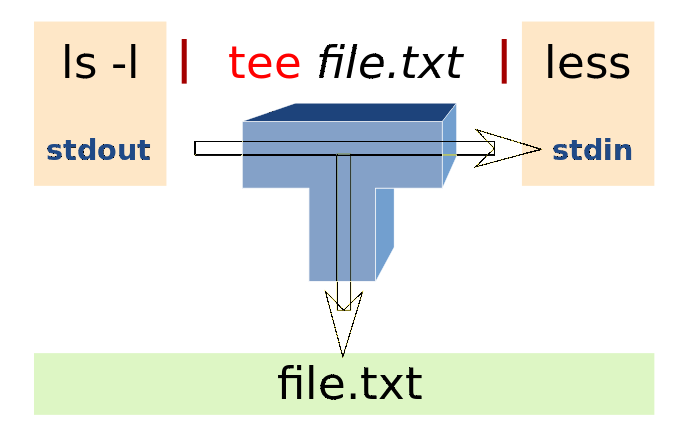
\includegraphics[width=0.5\textwidth]{pics/Tee2}\\
\footnotesize
Kép forrása: \url{http://hu.wikipedia.org/wiki/Tee_\%28parancs\%29}
\end{center}

\subsubsection*{Példa (1)}
Nézzünk a csővezeték és a \verb.tee. együttes használatára egy példát! Tegyük fel, hogy van egy fájlunk, melynek minden sorában egy név áll. A \verb.sort. parancs segítségével a \verb@nevsor_kevert.txt@ tartalmát sorbarendezzük. A sorbarendezés eredménye a \verb.tee. parancs hatására megjelenik a standard kimeneten (terminál) illetve a \verb@nevsor.txt@ fájlban is.

\begin{lstlisting}
joe@localhost:~$ cat nevsor_kevert.txt 
Kocsis Attila
Dobi Imre
Toth Zoltan
Kormanyos Jozsef Sandor
Lok Arpad
Botas Zoltan
Baranyi Peter
Buza Endre Csongor
joe@localhost:~$ cat nevsor_kevert.txt |sort|tee nevsor.txt
Baranyi Peter
Botas Zoltan
Buza Endre Csongor
Dobi Imre
Kocsis Attila
Kormanyos Jozsef Sandor
Lok Arpad
Toth Zoltan
\end{lstlisting}


\subsubsection*{Példa (2)}
%\begin{minipage}{0.7\textwidth}

\begin{lstlisting}
joe@localhost:~/tmp/Documents$ ls
BatteryLinux.png  final.png  Judy.png  pepita_sakk.png  ubigraph2.png
fajl.txt          hello.sh   Logo.png  ubigraph1.png
joe@localhost:~/tmp/Documents$ ls | tee fajl.txt
BatteryLinux.png
fajl.txt
final.png
hello.sh
Judy.png
Logo.png
pepita_sakk.png
ubigraph1.png
ubigraph2.png
joe@localhost:~/tmp/Documents$ cat fajl.txt 
BatteryLinux.png
fajl.txt
final.png
hello.sh
Judy.png
Logo.png
pepita_sakk.png
ubigraph1.png
ubigraph2.png
\end{lstlisting}

%\end{minipage}
%\begin{minipage}{0.25\textwidth}

%\end{minipage}


%\clearpage

\subsection{Szöveg kiírása, szöveges fájlok kezelése}
\Ovalbox{\large \texttt{echo} -- kiír egy szövegsort}
	\begin{quotation}
  Az   \verb.echo.  kiír  minden  megadott  karakteláncot a szabványos kimenetre,
       szóközökkel elválasztva és egy újsor karakterrel a  végén,  hacsak  nem
       volt megadva a \verb.-n. opció.
\bigskip

\emph{Kapcsolók}
\begin{description}

\item[-n]   Nem írja ki a sor végére a soremelést karaktert.


\item[-e]    Engedélyezi  a  következő  speciális  karakterek  értelmezését a
              karakterláncokban:
              \begin{description}
              \item[$\backslash$a]     riadó (csengő)
              \item[$\backslash$b]     egy karakter törlése visszafelé
              \item[$\backslash$c]     nem ír ki újsor karaktert
              \item[$\backslash$f]     lapdobás
              \item[$\backslash$n]     új sor
              \item[$\backslash$r]     kocsi vissza
              \item[$\backslash$t]     vízszintes tab
              \item[$\backslash$v]     függőleges tab
              \item[$\backslash\backslash$]     backslash
              \item[$\backslash$nnn]   a karakter ASCII kódja nnn (oktálisan)
              \end{description}

\item[-E]    backslash ($\backslash$) karakterrel megadott karakterek értelmezésének tiltása (alapértelmezett)
\end{description}

\begin{lstlisting}
joe@localhost:~$ echo "Hi all"
Hi all
joe@localhost:~$ echo 'Hi all!'
Hi all!
\end{lstlisting}

\end{quotation}

\clearpage

\noindent\Ovalbox{\large \texttt{printf} -- formátumozott adatkiírás}

   \begin{quotation}
      A printf kinyomtatja a formátum szöveget, értelmezi a '\%' és '$\backslash$' escape
       szekvenciákat ugyanúgy, mint a C \texttt{printf} függvény.  A formátum  argumentumot használja az összes kapott argumentum formázásához.
       
\begin{lstlisting}
joe@localhost:~$ printf "%s\n" "Hello World"  
Hello World
\end{lstlisting}
       \end{quotation}
\bigskip


\noindent\Ovalbox{\large \texttt{wc} -- fájlokban található bájtok, szavak és sorok számát írja ki}
	


\begin{quotation}
       A \verb.wc. program bájtok, szavak és újsor-jelek számát számolja meg az argumentumként megadott fájlokban.  Ha nem adunk meg fájlnevet,  illetve  a fájlnévként a '-' jelet adjuk meg, akkor a szabványos bemenet olvassa a program.

       Alapértelmezés szerint a \verb@wc@ mindhárom számot kiírja. Az opciókkal lehet megadni,  hogy csak bizonyos számok legyenek kiírva. Az opciók nem semlegesítik egymás hatását, így pl.  \verb@wc --bytes --words@  a  bájtok  és  a szavak számát egyaránt kiírja.  Minden fájlról egysornyi információt ír ki, és az argumentumként megadott fájlok nevét is kijelzi. Több fájlnév  esetén egy összesített sort is megad a lista végén \texttt{total} fájlnéven. A megadott adatok sorrendben a következőek: sorok, szavak, bájtok száma.
\bigskip

\textit{Kapcsolók}
\begin{description}
\item[-c, -{}-bytes, -{}-chars]
              Csak a bájtok számát írja ki.

\item[-l, -{}-lines]
              Csak a sorok számát írja ki.

\item[-w, -{}-words]
              Csak a szavak számát írja ki.

\item[-L, -{}-max-line-length]
              Csak a fájlban  előforduló  leghosszabb  sor  hosszát  írja  ki,
              illetve  ha  egynél  több  fájl volt megadva, akkor kiírja még a
              legnagyobbat az előző értékek közül (nem az összegüket írja ki).
\end{description}

\begin{lstlisting}
 joe@localhost:~$ wc os05.tex
  266  1152 11304 os05.tex
\end{lstlisting}

\end{quotation}
%\clearpage

\noindent\Ovalbox{\large \texttt{grep} -- mintához illeszkedő sorokat nyomtat}\footnote{A \texttt{grep} parancs neve a 
  \texttt{sed} parancs \texttt{/g/re/p} utasításából ered, ahol a \texttt{re} a regular expression rövidítése, A \texttt{grep} 
  ugyanis pontosan azt teszi, amit a \texttt{sed} erre az utasításra}

\begin{quotation}
 A \verb.grep. szétválasztja azokat a sorokat, amelyekben a keresett részlet megtalálható azoktól, melyekben nem. A grep alapesetben csak azokat a sorokat választja ki 
(írja ki), melyekben a keresett mintát megtalálta:
\begin{lstlisting}
joe@localhost:~$ ps -e|grep firefox
 3531 ?        00:11:22 firefox-bin
joe@localhost:~$ ps -e |grep kde
 3342 ?        00:00:00 kdeinit4
 3347 ?        00:00:00 kded4
\end{lstlisting}

A \texttt{-v} (revert, ellentétes) kapcsoló hatására a grep  csak azokat a sorokat tengedi tovább, melyekben a keresett
minta nem található meg. 

\begin{lstlisting}
joe@localhost:~$ who|grep joe
joe     tty7         2011-02-26 19:17 (:0)
joe     pts/0        2011-02-26 19:29 (:0.0)
joe     pts/3        2011-02-26 19:45 (:0.0)
joe     pts/1        2011-02-26 20:42 (:0.0)
joe     pts/2        2011-02-26 20:55 (:0.0)
joe@localhost:~$ who|grep -v pts
joe     tty7         2011-02-26 19:17 (:0)
\end{lstlisting}
A \texttt{-i} (ignore, figyelmen kívűl hagy) kapcsoló hatására a grep nem veszi figyelembe a kis- és nagybetűk közti különbséget.

\end{quotation}

%\clearpage

\noindent\Ovalbox{\large head --  fájlok első részének kiírása}
\begin{quotation}
A  \texttt{head}  a  megadott fájlok  első részét (alapértelmezésben első 10 sorát) írja ki. Ha nincs megadva fájlnév, vagy a fájlnév '-', a bemenetét  a  szabványos  bemenetről  veszi.  Ha  egynél  több fájl adott, a fájl nevét '==>' és '<=='
       jelek közé téve minden fájl első része előtt kiírja.
\bigskip

     A head kétfajta opciómegadást fogad el: az újat,  amikor  a  számok  az
       opciókat  jelző  betűknek  argumentumok  és  a  régit,  amikor a számok
       megelőzik az opciókat jelző betűket.

      \begin{description}
       \item[-c N, -{}-bytes N]
         Az első N bájtot írja ki. N nem-nulla egész,  amit  opcionálisan
              követ a következő karakterek közül egy, kijelölendő az egységet:

	    \begin{description}
	     \item[b] 512 bájt hosszú blokk
             \item[k] 1 kilobájt hosszú blokk
             \item[m] 1 megabájt hosszú blokk
	    \end{description}

      \item[-n N, -{}-lines N]
              Az első N sort írja ki.
      \end{description}
 
     
\end{quotation}

\noindent\Ovalbox{\large  \texttt{tail} -- kiírja a meghatározott fájl utolsó részét}

\begin{quotation}
 A tail parancs a megadott fájl(ok) utolsó sorait (10 sor  az  alapértelmezett) írja ki; a szabványos bemenetről olvas, ha nincs fájl megadva, vagy, ha
       a fájl nevet '-' követi.  Ha több, mint egy fájl van megadva, kiír  egy fejlécet, ami tartalmazza a fájl nevét '==>' és '<==' jelek közé zárva,
       a többi fájl kimenetei előtt.

  Kapcsolóit lásd a \texttt{head} parancsnál.
\end{quotation}

%\clearpage

\noindent\Ovalbox{\large \texttt{uniq} -- egy rendezett fájlból kiszedi a duplikált sorokat}
\begin{quotation}

       A \verb.uniq. kiírja az egyedi sorokat egy rendezett  fájlból,  és eldobja  az  egyezőket  egy  kivételével.  
      Opcionálisan,  mutathatja csak azokat a sorokat is, amelyek pontosan megegyeznek, illetve azokat, amelyek egynél többször fordulnak elő. A \verb.uniq.-nak rendezett bemenetre van  szüksége,  mivel
       csak az egymás után következő sorokat hasonlítja össze.

       Ha a kimenet nem specifikált, a \verb.uniq. a szabványos kimenetre ír. Ha a bemeneti file nincs megadva, 
	a standard input-ot  olvassa.
    \bigskip
    
    \emph{Kapcsolók}
    \begin{description}
     \item[-u, -{}-unique]
              Csak a nem azonos sorokat írja ki.

      \item[-d, -{}-repeated]
              Csak a duplikált sorokat írja ki.
    \end{description}
\end{quotation}


\noindent\Ovalbox{\large \texttt{dos2unix} -- szöveges fájlok átalakítására használható DOS/MAC $\rightarrow$ UNIX}

\begin{quotation}
    \emph{Fontosabb kapcsolók}
	\begin{description}
		\item[-k -\-keepdate] a kimeneti fájl időbélyege egyezni fog a bemenetivel
		\item[-c -\-convmode convmode] az átalakítás módja. Lehet: ASCII, 7bit, ISO, Mac, alapértelmezett az ASCII.
	\end{description}
\end{quotation}


\noindent\Ovalbox{\large \texttt{unix2dos} -- szöveges fájlok átalakítására használható UNIX $\rightarrow$ DOS/MAC}


\begin{quotation}
    \emph{Fontosabb kapcsolók}
	\begin{description}
		\item[-k -\-keepdate] a kimeneti fájl időbélyege egyezni fog a bemenetivel
		\item[-c -\-convmode convmode] az átalakítás módja. Lehet: ASCII, 7bit, ISO, Mac, alapértelmezett az ASCII.
	\end{description}
\end{quotation}


\subsection{Felhasználókkal kapcsolatos parancsok}
\noindent\Ovalbox{\large A \verb.who. parancs kilistázza a képernyőre a számítógépre bejelentkezett felhasználókat.}
%
\begin{quotation}
Amennyiben az opciókon kívül nincs argumentuma, a who program kinyomtatja minden, pillanatnyilag bejelentkezett felhasználóról a következő információkat:
\end{quotation}

\begin{itemize}
\item bejelentkezési név (login name) 
\item terminál vonal (terminal line) 
\item a bejelentkezés ideje (login time) 
\item távoli gépnév vagy X kijelző (remote hostname or X display)
\end{itemize}

\begin{lstlisting}
joe@localhost:~$ who
joe     pts/0        2011-02-19 11:03 (:0.0)
joe     pts/1        2011-02-19 12:03 (:0.0)
joe     pts/2        2011-02-19 12:04 (:0.0)
\end{lstlisting}

%Ha egyetlen argumentumot (amely nem opció) adunk meg a parancssorban, akkor a who program az így megadott fájlt használja a  /etc/utmp    helyett a bejelentkezett   felhasználók azonosítására. Szokás a   /etc/wtmp -t használni itt, hogy az előző bejelentkezéseket vizsgálhassuk. 


\noindent\Ovalbox{\large A \verb.whoami. parancs kiírja a felhasználó nevét.}
%
\begin{quotation}
A \texttt{whoami} program kiírja a bejelentkezett felhasználó nevét.
\end{quotation}
\begin{lstlisting}
joe@localhost:~$ whoami
joe
\end{lstlisting}



\noindent\Ovalbox{\large A \verb.finger. parancs a felhasználói információk megjelenítésére szolgál.}

\hfill\texttt{finger [user]}
\medskip

\textit{Kapcsolók}
\begin{description}
\item[-s] A finger megmutatja a felhasználó belépési nevét, valódi nevét, terminálját és hogy az írható-e (a terminál neve mögött ``* jelenik meg, ha nem írható), mióta nem csinált semmit, mikor lépett be, valamint irodájának helyét és telefonszámát. A belépés idejét hónap, nap, óra, perc formában adja meg, kivéve ha hat hónapnál régebben lépett be; ezesetben az óra és a perc helyett az évet jelzi ki. Az ismeretlen eszközök és a nemlétező belépési valamint nyugalmi időt csillaggal jelzi.

\item[-l] Többsoros megjelenítés, amely magában foglalja az \verb.-s. kapcsoló által mutatott adatokat, valamint a felhasználó home mappáját, otthoni telefonszámát, belépési shelljét, leveleinek állapotát és a home mappájában található \verb@.plan@, \verb@.project@ valamint \verb@.forward@ nevű fájlok tartalmát.
\end{description}

\begin{lstlisting}
joe@localhost:~$ finger
Login     Name            Tty     Idle  Login Time   Office     Office Phone
joe      Joe C.  	 pts/0       4  Feb 19 11:03 (:0.0)
joe      Joe C.  	 pts/1    1:05  Feb 19 12:03 (:0.0)
joe      Joe C.  	 pts/2          Feb 19 12:04 (:0.0)
\end{lstlisting}



